\subsection{Query Completion}
\label{sec:completion}

\begin{figure*}[t]
    \centering
    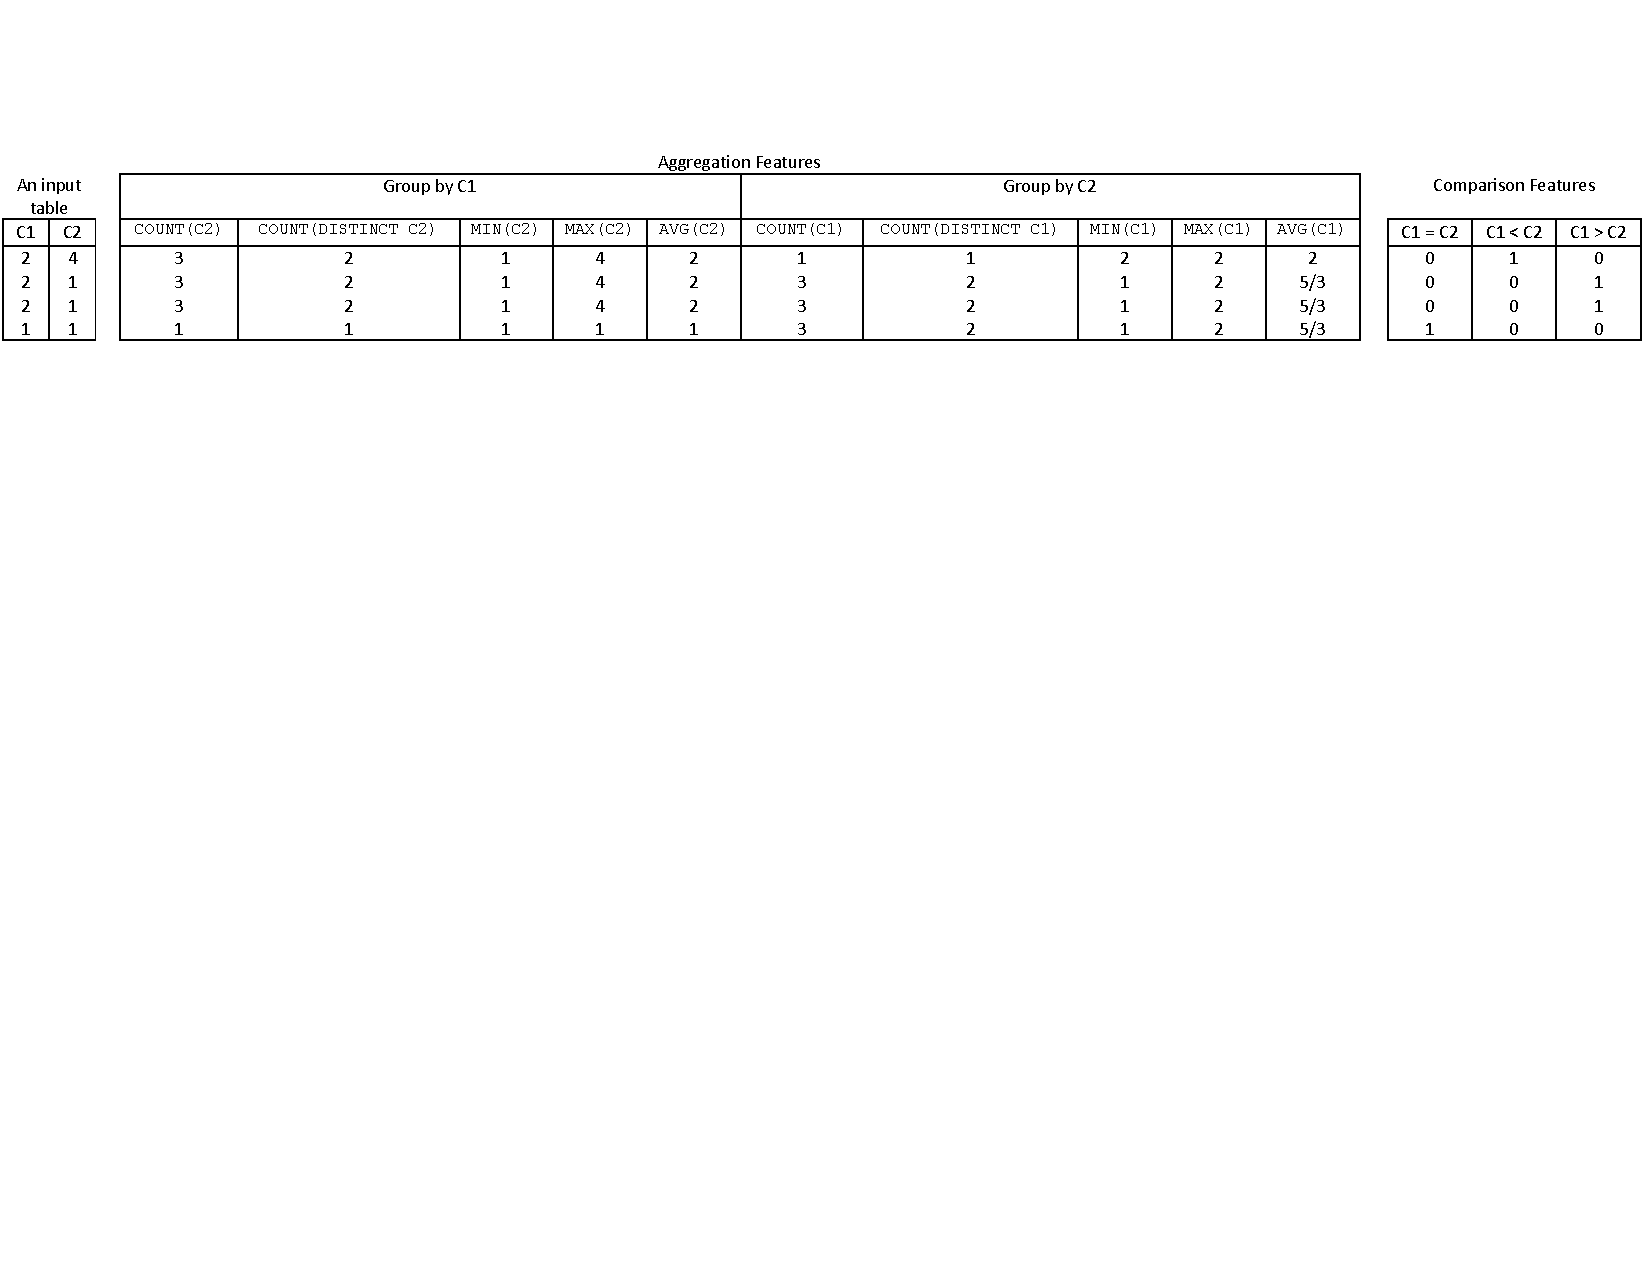
\includegraphics[scale=0.68]{featurex}
    \vspace{-7mm}
	\caption{Illustration of two additional features
    added by \ourtool. (Left) An example input table with
    two columns: C1 and C2. (Center) The aggregation features added by
    \ourtool for the input table. (Right) The comparison features
    added by \ourtool for the input table.
    Take the first row in the input table as an example,
    when grouping the table by column C1 (with value 2), the number
    of values in the C2 column is 3; the  number of
    distinct values in the C2 column is 2; the minimal value
    in the C2 column is 1, the maximal value in the C2 column
    is 4, and the average value in the C2 column is 2. Similar
    results can be computed if the table is grouped by the C2
    column.
}
	\label{fig:features}
\end{figure*}


In this step, \ourtool analyzes each created query skeleton
, and completes the missing query conditions (Section~\ref{sec:condition}),
aggregates (Section~\ref{sec:agg_search}), and
the \CodeIn{ORDER BY} clause (Section~\ref{sec:orderby}).
\ourtool outputs a list of syntactically-correct SQL queries
that satisfy the given example input and output.


%The SQL skeleton produced by the first step, though incomplete,
%serves as a good reference in inferring complete and valid SQL queries.
%In this step, our technique the remaining incomplete parts: conditions and
%aggregates, by rule-based learning and type-directed search, respectively.

\subsubsection{Inferring Query Conditions}
\label{sec:condition}

\ourtool casts the problem of \textit{inferring query conditions} as
 \textit{learning appropriate rules} that can perfectly divide a search space
into a positive part and a negative part. In our context, the search space
is all tuples from joining all query tables; the positive part
includes all tuples in the output table; and the negative part includes the rest
tuples.

The standard way for rule learning is using a decision-tree-based
algorithm. However, a key challenge
is how to design a good feature set.
Existing approaches~\cite{Tran:2009} simply use
tuple values in the input table(s) as features, 
and limits their abilities in inferring more
complex rules as query conditions. In particular,
merely using tuple values as features can only infer
conditions that compares a column value with a constant
(e.g., \CodeIn{student.level = 'senior'}), but
fails to infer conditions using aggregates (e.g., \CodeIn{COUNT(enrolled.course\_id) > 2}),
or conditions comparing the values of two table columns
(e.g., \CodeIn{enrolled.course\_id > enrolled.score}).
Figure~\ref{fig:fullexample} shows an example, in
which the expected query condition uses the \CodeIn{COUNT} aggregate.


\ourtool addresses this challenge by adding two types of
additional features to each tuple. When inferring rules, \ourtool
uses the existing tuple values and the newly-added features
together as the feature set.

\begin{itemize}

\item {\textbf{Aggregation Features}}. For each table column,
\ourtool groups all tuples by that column's value,
and then applies every applicable aggregate (i.e.,
\CodeIn{COUNT}, \CodeIn{COUNT DISTINCT}, \CodeIn{MAX},
\CodeIn{MIN}, and \CodeIn{AVG} for a numeric type column;
and \CodeIn{COUNT}, and \CodeIn{COUNT DISTINCT} for a string type column) to each
 \textit{remaining} column and computes the aggregation result. 
The ``Aggregation Features'' part in Figure~\ref{fig:features}
shows an example.

\item {\textbf{Comparison Features}}. For each tuple, \ourtool compares
the values of every two type-comparable columns, and records
the comparison results ($1$ or $0$) as features.
The ``Comparison Features'' part in Figure~\ref{fig:features}
shows an example.

\end{itemize}

%The above two additional features seamlessly encodes SQL
%structure
% knowledge encoding permits our technique
%to make use of correlations between columns, rather than only values
%from each isolated and sequential columns.
%Table~\ref{tbl:com} shows an example.

\todo{The incerasing number of features, can be falsified quickly}

Using both tuple values and the enhanced features,
\ourtool employs a variant of the decision tree algorithm,
called PART~\cite{Frank:1998}, to infer a set of rules
as query conditions.
Compared to the original decision tree algorithm~\cite{},
PART has two notable features.
First, it uses a ``divide-and-conquer'' strategy to repeatedly
construct rules and remove tuples that have already been covered until
no tuples are left, and thus is more efficient.
Second, when constructing each rule, PART uses a pruned decision
tree built from current set of tuples and only makes the leaf with
the largest coverage into the resulting rules, without keeping
the whole learned tree in memory.
This permits PART to consume less memory than the original decision
tree algorithm.




\begin{figure*}[t]
  \centering
  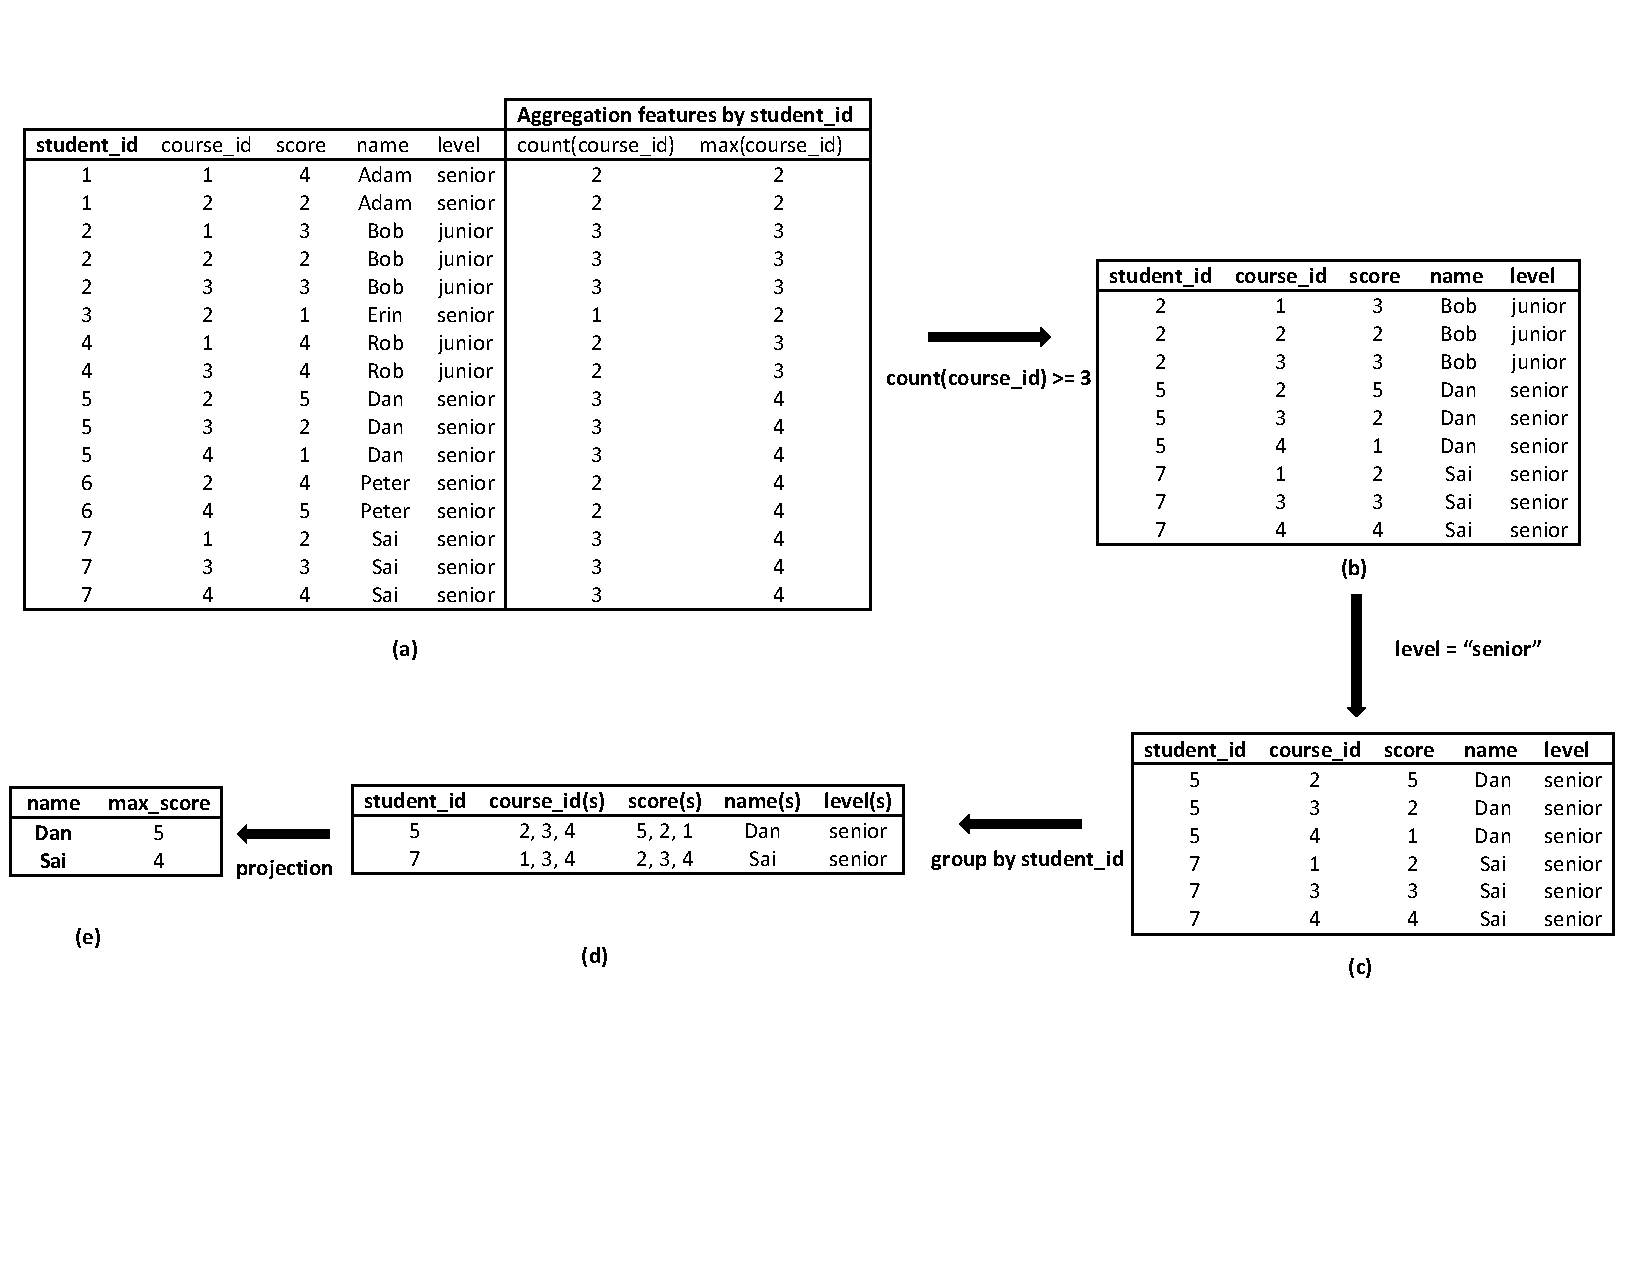
\includegraphics[scale=0.65]{fullexample}
  \vspace*{-5.0ex}\caption {{\label{fig:fullexample}
  Illustration of how additional features added by \ourtool
  helps in inferring query conditions. (a) shows \ourtool
  enriches the original table (Left: the
  result of joining table \CodeIn{student} with table
  \CodeIn{enrolled} on the \CodeIn{student\_id} column)
  with additional features. For brevity, only relevant
  aggregation features are shown. Using the added aggregation
  features, \ourtool infers two query conditions that
  transform the original table into the table show in (b).
  Note that, without the aggregation features enhanced by
  \ourtool, a learning algorithm will \textit{fail} to learn the above conditions.
  (c) shows the output table, which is produced by projecting the
   table in (b)
  on its column: name, and an aggregate: \CodeIn{MAX}(score).
}}

\end{figure*}


\ourtool next splits the inferred rules into two parts:
it puts conditions using aggregates to the \CodeIn{HAVING}
clause and puts other conditions to the \CodeIn{WHERE} clause.
This is becuase according to the SQL specification,
query conditions using aggregates are valid only when they
are used \textit{after} the \CodeIn{GROUP BY} clause.
For the example conditions inferred in Figure~\ref{fig:fullexample},
\ourtool puts \CodeIn{student.level =`senior'}
to the query condition part in the \CodeIn{WHERE} clause,
\CodeIn{COUNT(enrolled.course\_id) > 2} to the
query condition part in the \CodeIn{HAVING} clause,
column \CodeIn{student\_id} to the \CodeIn{GROUP BY} clause.

%\smallskip





%\end{itemize}

\subsubsection{Searching for Aggregates}
\label{sec:agg_search}

For each column that is produced by an aggregate,
\ourtool repeatedly applies each applicable aggregate on
every type-compatible table column to test its correctness.
\ourtool adapts two rules to reduce the search space:
%To discard 
%the whole search space includes all possible combinations
%of table columns and the five supported aggregation operators (see Figure~\ref{fig:syntax}).
%\ourtool leverages the following two observations to
%further reduce the search space:

\begin{itemize}
\item The data values in an output column must be compatible with an
aggregator's return type. For instance, if an output column
contains float values, it cannot be produced by using \CodeIn{COUNT}
or \CodeIn{COUNT DISTINCT}, or it cannot be produced by
using the \CodeIn{MAX} aggregator over a column with Integer type.
%has the String type, it must not use aggregation operators (e.g.,
%\CodeIn{count} and \CodeIn{sum}) that returns
%an Integer. 

\item When using the \CodeIn{MAX} and \CodeIn{MIN} aggregator,
each value in the output column must appear in the input
table.
%such as \CodeIn{MAX} and \CodeIn{min},
%is used, each value in the output column must has appeared in the input table.
\end{itemize}

We found both rules are useful to speed up the search for appropriate
aggregates.
%In our experience, the type-directed searching strategy significantly reduces the
%searching space and makes our tool find the desirable aggregates faster.

%\todo{Order by structure, relatively each to add}
\subsubsection{Searching for columns in the \CodeIn{ORDER BY} column}
\label{sec:orderby}
\ourtool scans data values for each column of the output table. If
the data values in a column are sorted, \ourtool
append the column name to the \CodeIn{ORDER BY} clause.
